\chapter{Workout Generation} \label{workout}\index{workout}
\pagestyle{fancy}

\section{MIA Workout Generation Overview and Introduction}

The workout generation in MIA is created for producing a workout with customization from the user. The generation of a workout within MIA has some dependencies on random value generation and thus is capable of creating different workouts each run. MIA is also capable of creating an entire weeks worth of workouts and outputting it to a file for the user. The entire generation process depends on a few input values, such as maximum number of sets, maximum number of exercises per set, and more which are all defined in a exercises file. Upon running the workout generation, the user enters a difficulty and MIA generates a workout with appropriate difficulty based on this number and the input file (see section \ref{workout algorithm} for more details).  

Throughout this section, workout can be defined as the complete output generated by MIA containing some number of sets, some number of exercises per set, and some number of reps per exercises.

\section{Input File and Defining Workouts}

\subsection{Input File}

The MIA workout generation utilizes an input file to determine exercises, exercise weighted values and various generation values. By default, this file is located in ../bin/Resources/InputFiles/exercises.txt but this file name and path can be changed via the MIAConfig file (see section \ref{MIAConfig} for more details). The contents of this input file look similar to the following.

\lstset{language=Python}

\begin{lstlisting}
#============================================================================
# Name        : exercises.txt
# Author      : Antonius Torode
# Date        : created on 3/14/18
# Copyright   : This file can be used under the conditions of Antonius' 
#               General Purpose License (AGPL).
# Description : Different workouts with weighted values for workout generation.
#============================================================================

# Various comments blocks explaining usage.
# ...
# ...
toughness = 0.1
minNumOfExercises = 3.0
maxNumOfExercises = inf
minNumOfSets = 1.0
maxNumOfSets = inf

# Exercises and weights.
push_up = 8.0; reps
sit_up = 15.0; reps
pull_up = 0.75; reps
squat = 3.0; reps
jumping_jack = 30.0; reps
\end{lstlisting}

This file must be in the correct format in order for the MIA workout generation to function properly. First, commented lines are created using the '\#' character. These lines are ignored by MIA when running internal algorithms. Within this input file, spaces are not important. Upon initialization, the MIA program will ignore all spaces within this file. Next, there are a few variables that the user can customize and define within this file which are below.

\subsection{Workout Generation Parameters}

\begin{lstlisting}
toughness = 0.1
minNumOfExercises = 3.0
maxNumOfExercises = inf
minNumOfSets = 1.0
maxNumOfSets = inf
\end{lstlisting}

These values must appear in the input file before any defined exercises. To begin, toughness is a global variable that helps define the number of reps MIA will output per workout chosen. Increasing this value is a global increase to the workout generation difficulty. The default value for toughness is 0.1 (see section \ref{workout algorithm} for more details). Next, There are minNumOfExercises\index{minNumOfExercises} and maxNumOfExercises\index{maxNumOfExercises} variables which are used to determine the minimum number of exercises MIA will choose per set and the maximum number of exercises MIA can choose per set. The maxNumOfExercises value is read in such that a value of 'inf' is allowed. If 'inf' is selected, MIA will set the total number of exercises within the input file to be the maximum. Similarly, there are minNumOfSets\index{minNumOfSets} and maxNumOfSets\index{maxNumOfSets} values which work in identical ways to minNumOfExercises\index{minNumOfExercises} and maxNumOfExercises\index{maxNumOfExercises} only defining a minimum and maximum for number of sets per generated workout instead of number of exercises per set. 

\begin{note}
	At the time of writing this, the MIA program is not designed to account for a value of maxNumOfExercises that is larger than the actual number of exercises defined in the input file.
\end{note}

\subsection{Defining Exercises}

Following these program variables, the main part of the input file is the defined exercises. The exercises are defined similar to below.

\begin{lstlisting}
# Exercises and weights.
push_up = 8.0; reps
sit_up = 15.0; reps
pull_up = 0.75; reps
squat = 3.0; reps
running = 0.1; mile
jumping_jack = 30.0; reps
\end{lstlisting}

Each exercise is defined using a common form. As shown below, the line must begin with an exercise name. Following this comes an equal sign and then a weighted value. This weighted value is defined to be relative to all other weighted values. This mean that in the above example, the file is claiming 8.0 push ups are equivalent to 15.0 sit ups, and similarly, 0.75 pull ups, etc. The MIA program will assume and each weight value for each exercise is of the same real world difficulty to the user. Following the weighted value must come a semi-colon and then a unit. The equal sign and semi-colon are important because they define how MIA separates the values. As stated previously, spaces are irrelevant in these definitions (See below).

\begin{lstlisting}
# Proper format for definind an exercise in the input file.
exercise_Name = exercise_Weighted_Value; exercise_Unit

#The following three lines are equivalent when read in by MIA.
pull ups = 15.0; reps
pullups=15.0;reps
p   ull u ps   =   15  . 0   ; reps
\end{lstlisting}


\section{Generation Algorithm}\label{workout algorithm}

This section contains an outline of the algorithm used to generate the MIA workouts. The MIA generation is based on creating two curves (maximum and minimum) for a parameter and then deciding upon which parameter to use for a workout by taking a random value between both curves. For the purposes of this section, we will denote a random number between two values $q_1$ and $q_2$ as $rand[q_1,q_2]$. We will denote a complete workout with $W$.

\subsection{Number of Sets Per Workout}

The number of sets, denoted $S(s_{min},s_{max},d) \equiv S$ is dependent on three variables. The first two are from the input file which are minNumOfSets, denoted $s_{min}$ and minNumOfSets, denoted $s_{max}$. The last is the difficulty $d$ which is input by the user upon generation. The maximum number of sets was originally based on a linear increase, however for better optimization of the real world workout difficulties, a custom algorithm was created. The maximum $S_{max}(s_{min},s_{max},d)$ and minimum $S_{min}(s_{min},s_{max},d)$ number of sets per workout are given by
\begin{align}
S_{max}(s_{min},s_{max},d) \equiv S_{max}&= \frac{s_{max}-s_{min}}{10^{4/3}} d^{2/3}+s_{min} \\
S_{min}(s_{min},s_{max},d) \equiv S_{min}&= \frac{s_{max}-1.9 \times s_{min}}{1.9 \times 10^{4/3}} d^{2/3}+s_{min}.
\end{align}
Thus since $S(s_{min},s_{max},d)$ is a random value between these curves, we have
\begin{align}
S_{ave}(s_{min},s_{max},d) \equiv S_{ave} &= \frac{S_{max}+ S_{min}}{2} \\ &= \frac{\left(2.9s_{max}-3.8s_{min}\right)}{3.8 \times 10^{4/3}}d^{2/3}+s_{min} \\
S(s_{min},s_{max},d) &= rand[S_{min}(s_{min},s_{max},d),S_{max}(s_{min},s_{max},d)].
\end{align}
These are shown in Figure \ref{Svd and Evd}. The algorithm used to determine the sets per workout is identical to that of determining the number of exercises per set.

\begin{figure}[h]
	\centering
	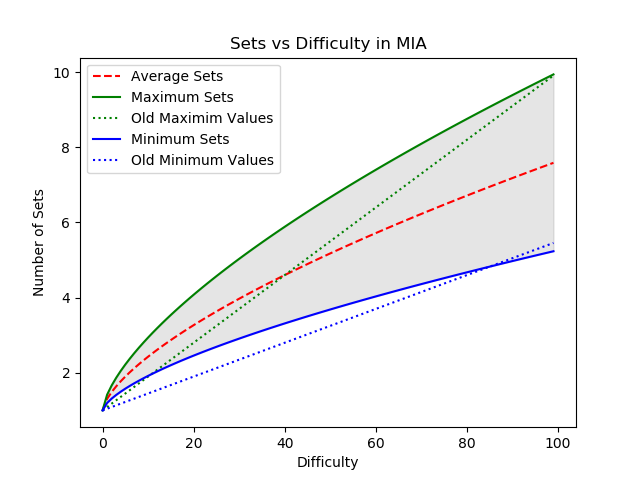
\includegraphics[width=0.5\textwidth]{images/Svd.png}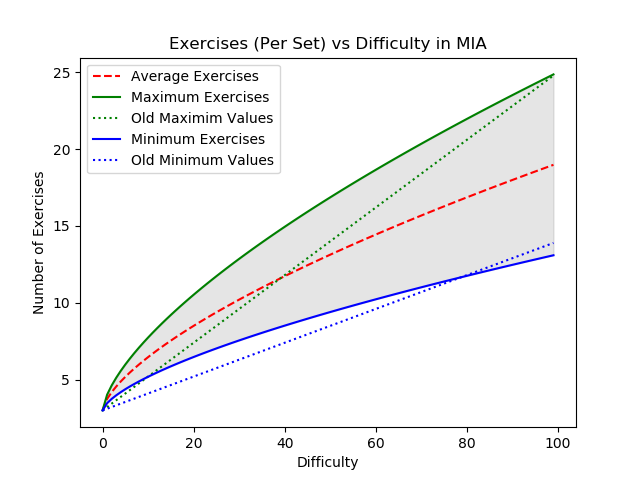
\includegraphics[width=0.5\textwidth]{images/Evd.png}
	\caption{Number of sets per workout (left) and number of exercises pet set (right) based on the user input difficulty. The small dotted lines represent the original algorithm which was a simple linear increase in difficulty for each parameter. For the above two figures, values of $s_{min}=1.0$, $s_{max} = 10.0$, $e_{min}=3.0$ and $e_{max}=25.0$ were used. The possible values for $S$ and $E$ are shown via the gray shaded areas.} \label{Svd and Evd}
\end{figure}

\subsection{Number of Exercises Per Set}

The number of exercises, denoted $E(e_{min},e_{max},d) \equiv E$ is dependent on three variables. The first two are from the input file which are minNumOfExercises\index{minNumOfExercises}, denoted $e_{min}$ and maxNumOfExercises\index{maxNumOfExercises}, denoted $e_{max}$. The last is the difficulty $d$ which is input by the user upon generation. The maximum number of sets was originally based on a linear increase, however for better optimization of the real world workout difficulties, a custom algorithm was created. The maximum $E_{max}(e_{min},e_{max},d)$ and minimum $E_{min}(e_{min},e_{max},d)$ number of sets per workout are given by
\begin{align}
E_{max}(e_{min},e_{max},d) \equiv E_{max}&= \frac{e_{max}-e_{min}}{10^{4/3}} d^{2/3}+e_{min} \\
E_{min}(e_{min},e_{max},d) \equiv E_{min}&= \frac{e_{max}-1.9 \times e_{min}}{1.9 \times 10^{4/3}} d^{2/3}+e_{min}.
\end{align}
Thus since $E(e_{min},e_{max},d)$ is a random value between these curves, we have
\begin{align}
E_{ave}(e_{min},e_{max},d) \equiv E_{ave} &= \frac{E_{max}+ E_{min}}{2} \\ &= \frac{\left(2.9e_{max}-3.8e_{min}\right)}{3.8 \times 10^{4/3}}d^{2/3}+e_{min} \\
E(e_{min},e_{max},d) &= rand[E_{min}(e_{min},e_{max},d), E_{max}(e_{min},e_{max},d)].
\end{align}
These are shown in Figure \ref{Svd and Evd}. Since this value depends on each set, and there are generally numerous sets per workout, we denote the set within the workout with $i$ such that $1\leq i \leq S$, where $S$ is the total number of sets within a workout. Using this index, $E_i$ becomes
\begin{align}
	E_{i,max}(e_{min},e_{max},d) \equiv E_{max}&= \frac{e_{max}-e_{min}}{10^{4/3}} d^{2/3}+e_{min} \\
	E_{i,min}(e_{min},e_{max},d) \equiv E_{min}&= \frac{e_{max}-1.9 \times e_{min}}{1.9 \times 10^{4/3}} d^{2/3}+e_{min} \\
	E_{i,ave}(e_{min},e_{max},d) \equiv E_{ave} &= \frac{E_{max}+ E_{min}}{2} \\ &= \frac{\left(2.9e_{max}-3.8e_{min}\right)}{3.8 \times 10^{4/3}}d^{2/3}+e_{min} \\
	E_i(e_{min},e_{max},d) &= rand[E_{i,min}(e_{min},e_{max},d), E_{i,max}(e_{min},e_{max},d)].
\end{align}
Following this, the average number of exercises done for a given workout would be
\begin{align}
	E_{W} = \frac{1}{S}\sum_{i=1}^{S}E_i.
\end{align}

\begin{figure}[h]
	\centering
	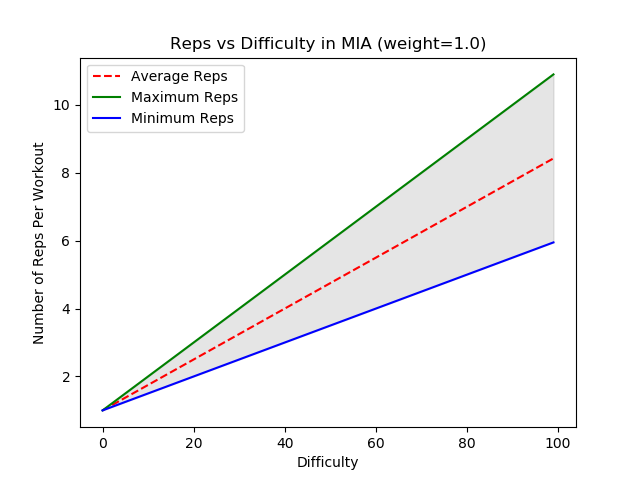
\includegraphics[width=0.5\textwidth]{images/Rvd1.png}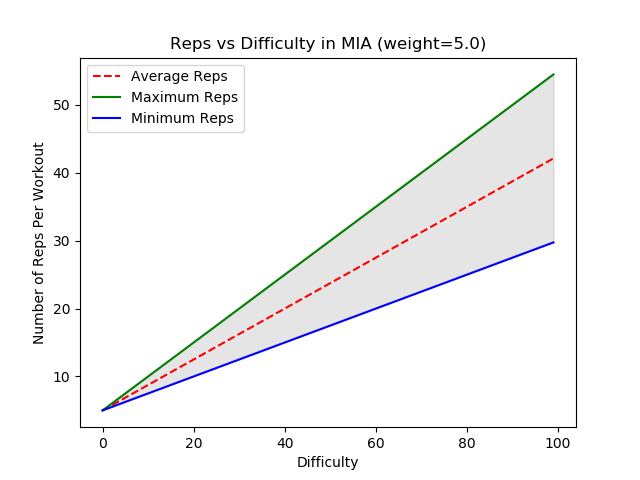
\includegraphics[width=0.5\textwidth]{images/Rvd5.png}
	\caption{Number of reps per exercise. On the right, we have $R(0.1,d,1)$ and on the left, $R(0.1,d,5)$. The possible values for $R$ are shown via the gray shaded area.} \label{Rvd}
\end{figure}


\subsection{Number of Reps Per Exercise}

The number of reps, denoted $R(t,d,w) \equiv R$ is dependent on three variables. The first is toughness $t$ which is gathered from the input file or defaults to 0.1. The second is difficulty $d$ which is input by the user upon generation. Lastly, the weight $w$ of a given exercise is needed to provide the total reps that are output. The reps are determined by a linear trend given by
\begin{align}
	R_{max}(t,d,w) &= tdw+w \\
	R_{min}(t,d,w) &= \frac{tdw}{2}+w \\
	R_{ave}(t,d,w) &= \frac{R_{max}+R_{min}}{2} = \frac{3tdw}{4}+w \\
	R(t,d,w) &= rand[R{min}(t,d,w),R_{max}(t,d,w)].
\end{align}
These are shown in Figure \ref{Rvd}. Since this value depends on each exercise, and there are generally numerous exercises per set, we denote the exercises within the set by an index $j$ such that $1 \leq j \leq E_i$, where $E_j$ is the total number of exercises within the given set $i$. Using this index, $R$ becomes
\begin{align}
	R_{j,max}(t,d,w_j) &= tdw_j+w_j \\
	R_{j,min}(t,d,w_j) &= \frac{tdw_j}{2}+w_j \\
	R_{j,ave}(t,d,w_j) &= \frac{R_{max}+R_{min}}{2} = \frac{3tdw_j}{4}+w_j \\
	R_j(t,d,w_j) &= rand[R_{j,min}(t,d,w_j),R_{j,max}(t,d,w_j)].
\end{align}
Following this, the average number of normalized reps done per set would be
\begin{align}
	R_{i,ave} = \frac{1}{E_i}\sum_{j=1}^{E_i}\frac{R_j}{w_j}.
\end{align}
Then, the average number of reps (normalized by the weights) done per workout would be given by
\begin{align}
	R_{W} = \frac{1}{S}\sum_{i=1}^{S}\frac{1}{E_i}\sum_{j=1}^{E_i}\frac{R_j}{w_j}
\end{align}

\section{Real World Difficulties} 

Due to the way that we set up the weighted system for each exercise, we can easily determine how difficult, denoted $D$ a workout is in reality based upon the generation. First, a workout is directly proportional to the number of sets it contains and thus $D \propto S$. Similarly, the difficulty of each set is proportional to the number of exercises are contained within each set and thus we use $D \propto E_{W}$. Lastly, the difficulty of each exercise is proportional to the number of normalized reps, and thus $D \propto E_{W}$. By combining all of these components we get
\begin{align}
	D \equiv S E_{W} R_{W} = S \left(\frac{1}{S}\sum_{i=1}^{S}E_i \right)\frac{1}{S}\sum_{i=1}^{S}\frac{1}{E_i}\sum_{j=1}^{E_i}\frac{R_j}{w_j}.
\end{align}

To demonstrate the possible values that can be output by $D$ we can examine the maximum and minimum values. The maximum value would be when $S$, $E$, and $R$ are at their maximums. Thus, we have
\begin{align}
	D_{max} &= S_{max} \left(\frac{1}{S_{max}}\sum_{i=1}^{S_{max}}E_{i,max} \right)\frac{1}{S_{max}}\sum_{i=1}^{S_{max}}\frac{1}{E_{i,max}}\sum_{j=1}^{E_{i,max}}\frac{R_{j,max}}{w_j}.
\end{align}
Since each $E_{i,max}$ and $R_{j,max}/w_j$ are the same for all $i,j$ respectively, then we can simplify this to
\begin{align}
	D_{max} &= S_{max} \left(\frac{1}{S_{max}}S_{max}E_{max} \right)\frac{1}{S_{max}}S_{max}\frac{1}{E_{max}}E_{max}\frac{R_{max}}{w} \\
	&= S_{max} E_{max} \frac{R_{j,max}}{w_j}.
\end{align}
Similarly, the minimum value is 
\begin{align}
	D_{min} = S_{min} E_{min} \frac{R_{j,min}}{w_j},
\end{align}
where $R_{j,min}/w_j$ represents the normalized reps for each exercise in both of the above two cases. The possible values of $D$ then lie between these two curves and can be seen in figure \ref{Dvd}.

\begin{figure}[h]
	\centering
	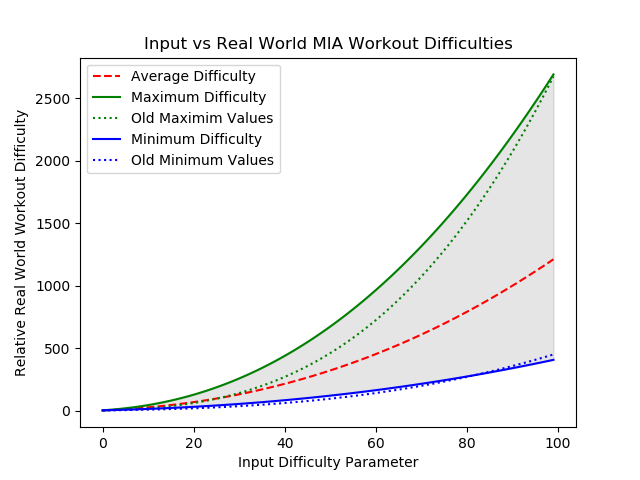
\includegraphics[width=0.5\textwidth]{images/Dvd.png}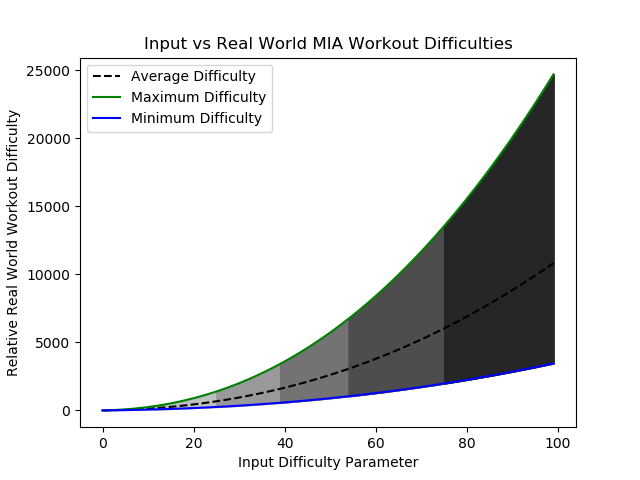
\includegraphics[width=0.5\textwidth]{images/Dvdc.png}
	\caption{The real world difficulties $D$ output by the MIA workout generation program versus the input difficulty parameter (LEFT). The possible values for $D$ are shown via the gray shaded area. The old min/max values represent $D$ based on the old $S$ and $E$ values (see figure \ref{Svd and Evd}). On the right is the same plot only depicting the difficulty ranges. The ranges run from very easy (light gray), to very hard (dark gray).} \label{Dvd}
\end{figure}

The real world difficulty $D$ has an exponential increase. This is desired for a specific reason. As improvements are made, meaning as ones physique and ability to perform improves, a greater challenge is needed. Similarly, there is a much larger variance in the real world difficulty $D$ increases with respect to the input difficulty $d$. This is because as workout intensities increase, there is a desire to keep the body both guessing and not straining too often. Therefore, by increasing the variability of a workout, there is a greater effectiveness and an improved 'rest' or 'slow' period between intensive workouts. 

\section{Notes on Appropriate MIA Parameters For Usage}

Based on the way MIA generates workouts (as described in the above sections), there are a few things to keep in mind when determining the proper settings. First, if a maxNumberOfExercises value of 'inf' is used, then the real world difficulty output will be proportional to the number of exercises defined in the input file. Therefore, if one places a thousand different workouts in this file, each difficulty will be drastically more intense than if there were only 25. Thus, it is important to experiment with this value and adjust accordingly based on the number of defined exercises you have in the input file.

 


